\documentclass{examen}
\usepackage{listings}
\begin{document}

\modulo{Lenguajes de marcas -- PARTE ESCRITA (PARTES 1 y 2)}

\pregunta{Crea un formulario como el mostrado en la figura}{2}
\begin{figure}[h]
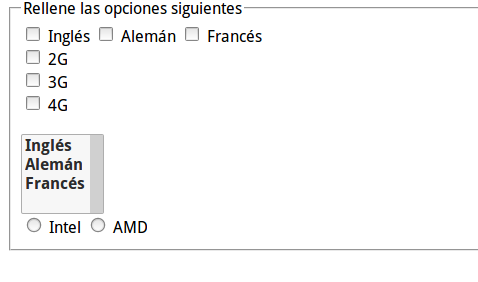
\includegraphics[scale=0.7]{examen-img/pagina.png}
\end{figure}

\break
\pregunta{Dado el archivo XML que se puede encontrar a continuaci�n, 
crear una hoja de estilo XSLT que transforme dicho archivo en el archivo XML que aparece al final. Observa que en el resultado solo aparecer� un producto {\bf si est� en el edificio A}
}{3.5}
\begin{verbatim}
<inventario><!--Archivo original-->
    <producto codigo="P1">
        <peso unidad="kg">10</peso>
        <nombre>Ordenador</nombre>
        <lugar edificio="B">
            <aula>10</aula>
        </lugar>
    </producto>
    <producto codigo="P2">
        <peso unidad='g'>500</peso>
        <nombre>Switch</nombre>
        <lugar edificio="A">
            <aula>6</aula>
        </lugar>
    </producto>
</inventario>
\end{verbatim}
\begin{verbatim}
<!--Esto debe ser lo que devuelva el archivo XSLT-->
<resultado>
    <producto codigo="P2">
        <peso>500 g</peso>
        <nombre>Switch</nombre>
        <ubicacion>A6</ubicacion>
    </producto>
</resultado>

\end{verbatim}

\end{document}
